%%%%%%%%%%%%%%%%%%%%%%%%%%%%%%%%%%%%%%%%%%%%%%%%%%%%%%%%%%%%%%%%%%%%%%%%%%%%%%%%%%%%%%%%%%%
%%%%%%%%%%%%%%%%%%%%%%%%%%%%%%%%%%%%%%%%%%%%%%%%%%%%%%%%%%%%%%%%%%%%%%%%%%%%%%%%%%%%%%%%%%%
%%%%%%%%%%%%%%%%%%%%%%%%%%%%%%%%%%%%%%%%%%%%%%%%%%%%%%%%%%%%%%%%%%%%%%%%%%%%%%%%%%%%%%%%%%%
\chapter{Результаты моделирования}
Данный раздел содержит результаты моделирвоания передачи данных при использовании каскадного
кодирования. Моделирование выполнялось с использованием разработанного и протестированного
приложения. Основная цель моделирования --- получение наглядных результатов, демонстрирующих
эффективность каскадного кодирования и корреллирующих с теоретическими ожиданиями, а также
оценка частоты появления ошибок на удаленной стороне.

%%%%%%%%%%%%%%%%%%%%%%%%%%%%%%%%%%%%%%%%%%%%%%%%%%%%%%%%%%%%%%%%%%%%%%%%%%%%%%%%%%%%%%%%%%%
%%%%%%%%%%%%%%%%%%%%%%%%%%%%%%%%%%%%%%%%%%%%%%%%%%%%%%%%%%%%%%%%%%%%%%%%%%%%%%%%%%%%%%%%%%%
%%%%%%%%%%%%%%%%%%%%%%%%%%%%%%%%%%%%%%%%%%%%%%%%%%%%%%%%%%%%%%%%%%%%%%%%%%%%%%%%%%%%%%%%%%%
\section{Передача изображения по системе моделирования}
На Рис.~\ref{img:experimoriginal} -- \ref{img:experimcoded12} представлены исходное изображение, моделирование передачи которого
производилось на программной модели. На вход поступают данные изображения, затем они искажаются в канале
в зависимости от текущих параметров канала. Далее искаженные данные принимаются на удаленной стороне и
декодируются. Под каждым изображением указаны параметры модели. Нотация параметров коррелирует с обозначением
ключей приложения, реализующего программную модель.

\begin{figure}[h]
\begin{center}
\begin{minipage}[h]{0.4\linewidth}
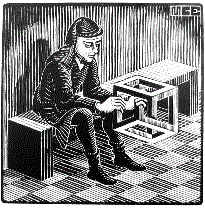
\includegraphics[width=1\linewidth]{chapter_4/img_test_01.png}
\caption{Исходное изображение} %% подпись к рисунку
\label{img:experimoriginal} %% метка рисунка для ссылки на него
\end{minipage}
\hfill 
\begin{minipage}[h]{0.4\linewidth}
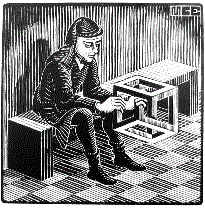
\includegraphics[width=1\linewidth]{chapter_4/img_test_01_transferred_g_4_l_15_e_3_d_31_b_0_000024.png}
\caption{g=4, l=15, e=3, d=31, b=0.000024}
\label{img:experimcoded2}
\end{minipage}
\end{center}

\begin{center}
\begin{minipage}[h]{0.4\linewidth}
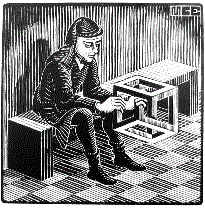
\includegraphics[width=1\linewidth]{chapter_4/img_test_01_transferred_g_4_l_15_e_3_d_31_b_0_009844.png}
\caption{g=4, l=15, e=3, d=31, b=0.009844}
\label{img:experimcoded3}
\end{minipage}
\hfill 
\begin{minipage}[h]{0.4\linewidth}
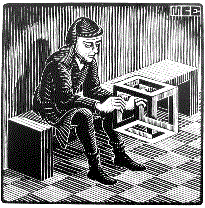
\includegraphics[width=1\linewidth]{chapter_4/img_test_01_transferred_g_4_l_15_e_3_d_31_b_0_011813.png}
\caption{g=4, l=15, e=3, d=31, b=0.011813}
\label{img:experimcoded4}
\end{minipage}
\end{center}
\end{figure}

\begin{figure}[h]
\begin{center}
\begin{minipage}[h]{0.4\linewidth}
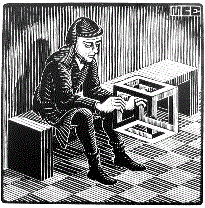
\includegraphics[width=1\linewidth]{chapter_4/img_test_01_transferred_g_4_l_15_e_3_d_31_b_0_014176.png}
\caption{g=4, l=15, e=3, d=31, b=0.014176}
\label{img:experimcoded5}
\end{minipage}
\hfill 
\begin{minipage}[h]{0.4\linewidth}
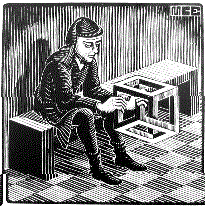
\includegraphics[width=1\linewidth]{chapter_4/img_test_01_transferred_g_4_l_15_e_3_d_31_b_0_017011.png}
\caption{g=4, l=15, e=3, d=31, b=0.017011}
\label{img:experimcoded6}
\end{minipage}
\end{center}

\begin{center}
\begin{minipage}[h]{0.4\linewidth}
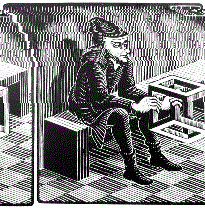
\includegraphics[width=1\linewidth]{chapter_4/img_test_01_transferred_g_4_l_15_e_3_d_31_b_0_020413.png}
\caption{g=4, l=15, e=3, d=31, b=0.020413}
\label{img:experimcoded7}
\end{minipage}
\hfill 
\begin{minipage}[h]{0.4\linewidth}
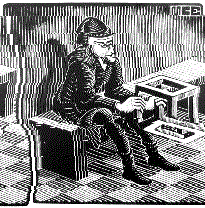
\includegraphics[width=1\linewidth]{chapter_4/img_test_01_transferred_g_4_l_15_e_3_d_31_b_0_024496.png}
\caption{g=4, l=15, e=3, d=31, b=0.024496}
\label{img:experimcoded8}
\end{minipage}
\end{center}
\end{figure}

\begin{figure}[h]
\begin{center}
\begin{minipage}[h]{0.4\linewidth}
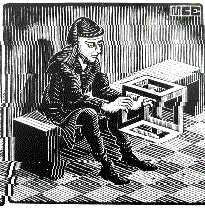
\includegraphics[width=1\linewidth]{chapter_4/img_test_01_transferred_g_4_l_15_e_3_d_31_b_0_029395.png}
\caption{g=4, l=15, e=3, d=31, b=0.029395}
\label{img:experimcoded9}
\end{minipage}
\hfill 
\begin{minipage}[h]{0.4\linewidth}
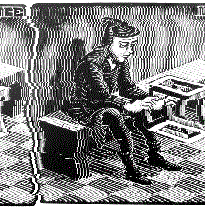
\includegraphics[width=1\linewidth]{chapter_4/img_test_01_transferred_g_4_l_15_e_3_d_31_b_0_035275.png}
\caption{g=4, l=15, e=3, d=31, b=0.035275}
\label{img:experimcoded10}
\end{minipage}
\end{center}

\begin{center}
\begin{minipage}[h]{0.4\linewidth}
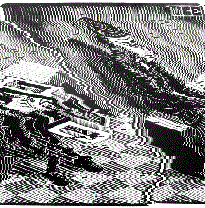
\includegraphics[width=1\linewidth]{chapter_4/img_test_01_transferred_g_4_l_15_e_3_d_31_b_0_042329.png}
\caption{g=4, l=15, e=3, d=31, b=0.042329}
\label{img:experimcoded11}
\end{minipage}
\hfill 
\begin{minipage}[h]{0.4\linewidth}
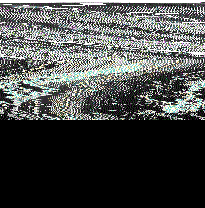
\includegraphics[width=1\linewidth]{chapter_4/img_test_01_transferred_g_4_l_15_e_3_d_31_b_0_060954.png}
\caption{g=4, l=15, e=3, d=31, b=0.060954}
\label{img:experimcoded12}
\end{minipage}
\end{center}
\end{figure}

Из данных рисунков видно, что приемлeмое качество изображения сохраняется даже при $BER=0.017011$, что говорит
о эффективности методов каскадного кодирования. При использовании $BER=0.020413$ изображение начинает содержать
искажения, которые увеличиваются при увеличении $BER$ соответственно. В реальной жизни, как правило, уровень ошибок в канале связи
гораздо меньше указанных значений (обычно он меньше $10^{-5}$). Это означает, что принятое изображение будет в таком случае примлемого
качества и пользователь на удаленной стороне практически не заметит разницу в случае, если даже при декодировании не удалось
восстановить исходную информацию.

Искажения изображений связаны с тем, что изображения изначально были представлены в формате GIF.
Формат способен хранить сжатые данные без потери качества в формате не более 256 цветов. Следовательно,
по причине того, что данные сжаты, при их повреждении наблюдается эффект искажения части изображения.
Для получения неразмытых изображений был использован формат BMP, отличающийся отсутствием кодирования данных.
На Рис.~\ref{img:bmp_experimcoded1} -- \ref{img:bmp_experimcoded4}  показаны исходное и переданные изображения.

\begin{figure}[h]
\begin{center}
\begin{minipage}[h]{0.4\linewidth}
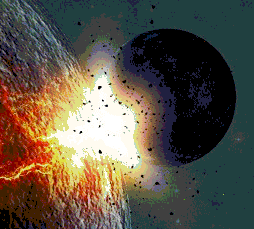
\includegraphics[width=1\linewidth]{chapter_4/img_test_05.png}
\caption{Исходное изображение}
\label{img:bmp_experimcoded1}
\end{minipage}
\hfill 
\begin{minipage}[h]{0.4\linewidth}
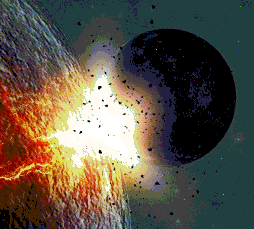
\includegraphics[width=1\linewidth]{chapter_4/img_test_05_transferred_g_4_l_15_e_3_d_31_b_0_020000.png}
\caption{g=4, l=15, e=3, d=31, b=0.02}
\label{img:bmp_experimcoded2}
\end{minipage}
\end{center}

\begin{center}
\begin{minipage}[h]{0.4\linewidth}
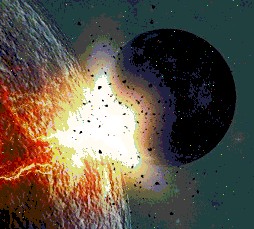
\includegraphics[width=1\linewidth]{chapter_4/img_test_05_transferred_g_4_l_15_e_3_d_31_b_0_040000.png}
\caption{g=4, l=15, e=3, d=31, b=0.04}
\label{img:bmp_experimcoded3}
\end{minipage}
\hfill 
\begin{minipage}[h]{0.4\linewidth}
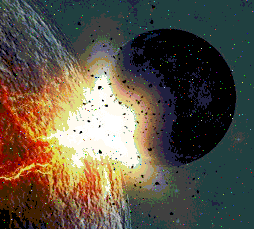
\includegraphics[width=1\linewidth]{chapter_4/img_test_05_transferred_g_4_l_15_e_3_d_31_b_0_050000.png}
\caption{g=4, l=15, e=3, d=31, b=0.05}
\label{img:bmp_experimcoded4}
\end{minipage}
\end{center}
\end{figure}

%%%%%%%%%%%%%%%%%%%%%%%%%%%%%%%%%%%%%%%%%%%%%%%%%%%%%%%%%%%%%%%%%%%%%%%%%%%%%%%%%%%%%%%%%%%
%%%%%%%%%%%%%%%%%%%%%%%%%%%%%%%%%%%%%%%%%%%%%%%%%%%%%%%%%%%%%%%%%%%%%%%%%%%%%%%%%%%%%%%%%%%
%%%%%%%%%%%%%%%%%%%%%%%%%%%%%%%%%%%%%%%%%%%%%%%%%%%%%%%%%%%%%%%%%%%%%%%%%%%%%%%%%%%%%%%%%%%
\section{Оценка частоты появления ошибок на удаленной стороне}
На Рис.~\ref{img_06} показана зависимость $BER$ на приемнике от $BER$ в канале при условии, что размер буфера накопленной
последовательности в узле решетки декодера Витерби составляет 1 фрейм (15 символов). На Рис.~\ref{img_07} и 
Рис.~\ref{img_08} показаны аналогичные зависимости, но при увеличении размера буфера до 2 и 10 фреймов соответственно.

\begin{figure}[h]
\begin{center}
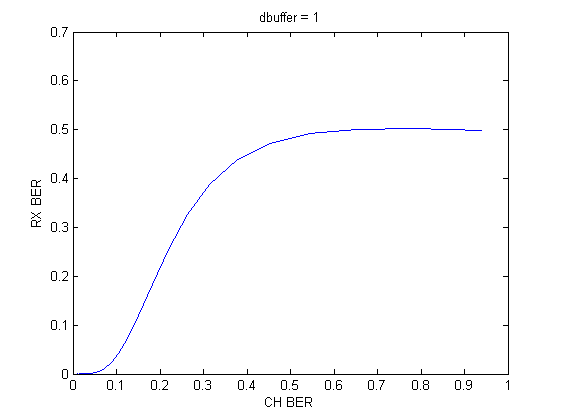
\includegraphics[width=0.7\linewidth]{chapter_4/matlab_img/dbuffer_1.png}
\caption{Зависимость BER на приемнике от BER в канале, dbuffer=1}
\label{img_06}
\end{center}
\end{figure}

\begin{figure}[h]
\begin{center}
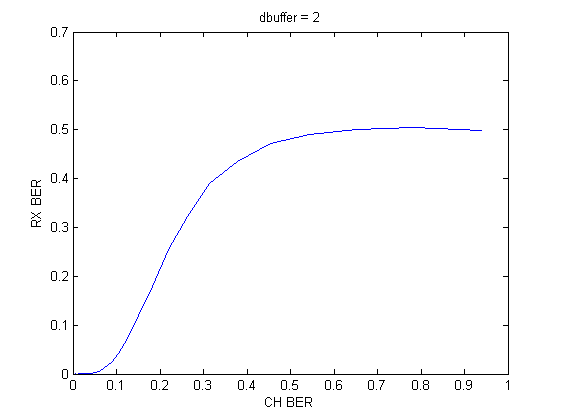
\includegraphics[width=0.7\linewidth]{chapter_4/matlab_img/dbuffer_2.png}
\caption{Зависимость BER на приемнике от BER в канале, dbuffer=2}
\label{img_07}
\end{center}
\end{figure}

\begin{figure}[h]
\begin{center}
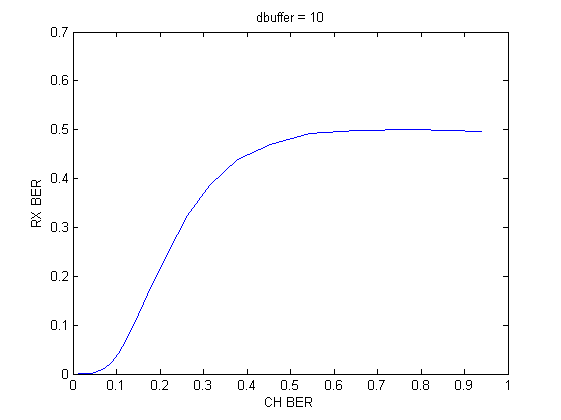
\includegraphics[width=0.7\linewidth]{chapter_4/matlab_img/dbuffer_10.png}
\caption{Зависимость BER на приемнике от BER в канале, dbuffer=10}
\label{img_08}
\end{center}
\end{figure}

На Рис.~\ref{img_09} показаны указанные зависимости совместно. Можно наблюдать, что в целом размер буфера накопленной
последовательности в узле решетки декодера Витерби не сильно влияет на поведение кривой.
\begin{figure}[h]
\begin{center}
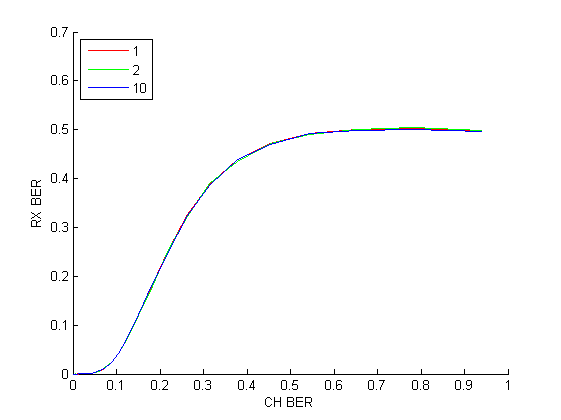
\includegraphics[width=0.7\linewidth]{chapter_4/matlab_img/all.png}
\caption{Зависимость BER на приемнике от BER в канале (все случаи)}
\label{img_09}
\end{center}
\end{figure}

На Рис.~\ref{img_10} показаны указанные зависимости совместно при низких значениях $BER$. На этих рисунках можно аналогично
наблюдать, что в целом размер буфера накопленной последовательности в узле решетки декодера Витерби не сильно влияет на поведение кривой.
\begin{figure}[h]
\begin{center}
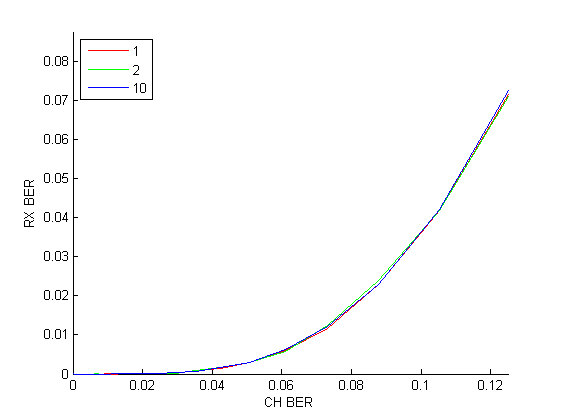
\includegraphics[width=0.7\linewidth]{chapter_4/matlab_img/all_01.png}
\caption{Зависимость BER на приемнике от BER в канале (все случаи)}
\label{img_10}
\end{center}
\end{figure}

На Рис.~\ref{img_11} показаны указанные зависимости в узком промежутке $BER$. На этих рисунках уже можно наблюдать, что размер буфера
накопленной последовательности в узле решетки декодера Витерби определенно влияет на поведение кривой. При увеличении размера
буфера уменьшается значение $BER$ на приемнике удаленной стороны. Это происходит потому, что в данном случае декодер Витерби
содержит большее количество накопленных символов для различных путей в решетке. Данные пути в этом случае с большей вероятностью
начинаются в одном узле и разветвляются по прошествии большего числа шагов. Следовательно, вероятность выдачи корректного символа выше.
\begin{figure}[h]
\begin{center}
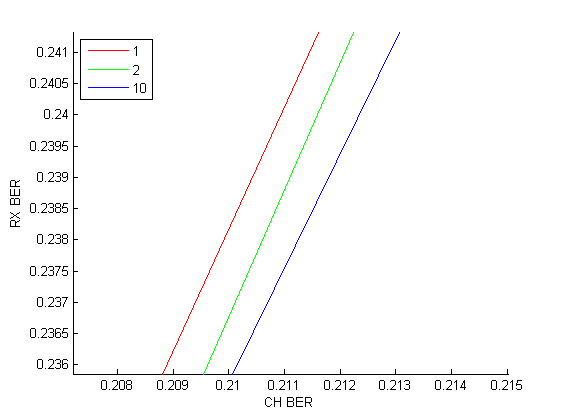
\includegraphics[width=0.7\linewidth]{chapter_4/matlab_img/all_02.png}
\caption{Зависимость BER на приемнике от BER в канале (все случаи)}
\label{img_11}
\end{center}
\end{figure}

Для получения теоретических результатов и сравнения с ними результатов, полученных на практике был выполнен следующий
эксперимент. Выполнялось моедлирование передачи данных при отключенном БЧХ-кодировании/декодировании, то есть использовалось
только сверточное кодирование и декодирование по алгоритму Витерби. Данная конфигурация обусловлена тем, что достаточно
просто (для использовавшегося сверточного кодера) построить верхнюю оценку зависимости $BER$ на приемнике от $BER$ в канале.

Указанные зависимости в логарифмическом масштабе представлены на Рис.~\ref{img_12}. График черного цвета показывает кривую,
получающуюся в результате теоретических вычислений. Из данного рисунка можно наблюдать, что теоретический результат
(верхняя граница) близок к результатам, полу-ченным благодаря моделированию.
\begin{figure}[h]
\begin{center}
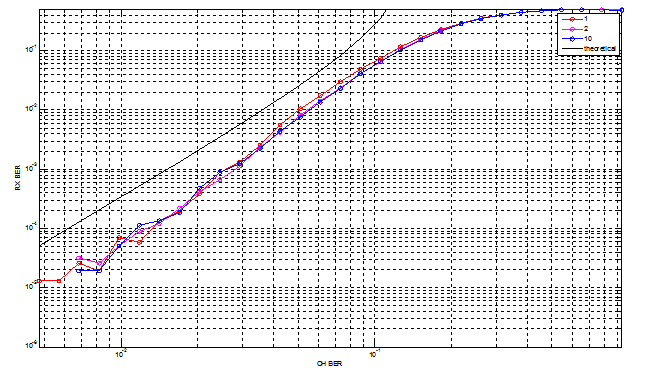
\includegraphics[width=0.8\linewidth]{chapter_4/matlab_img/all_log_theory.png}
\caption{Верхняя граница и полученные на практике результаты (БЧХ-кодирование/декодирование не используется)}
\label{img_12}
\end{center}
\end{figure}

Данный результат полностью согласуется с теорией. Более того, по предыдущим иллюстрациям можно наблюдать, что
зависимость уменьшения $BER$ на приемнике от применения буфера накопленной последовательности в узле решетки
декодера Витерби большего размера сохраняется.